\documentclass{article}
\usepackage{graphicx}
\usepackage{amsfonts}
\usepackage{amsmath}
\usepackage{amsthm}
\usepackage{bigfoot}
\usepackage{booktabs}
\usepackage{hyperref}
\usepackage{cleveref}
\usepackage{mathtools}
\usepackage{siunitx}
\usepackage{changes}

\usepackage{subcaption}
\usepackage{todonotes}
\usepackage{upgreek}
\usepackage{xcolor}

\usepackage[backend=biber,style=ieee]{biblatex}
\addbibresource{ref.bib}

\usepackage{fullpage}
\usepackage[modulo]{lineno}
\linenumbers

\title{LLR 2026: Lab 1 Report}
\author{Valentina Schüller}
\date{\today}

\begin{document}

\maketitle

The code is available at
\url{https://github.com/valentinaschueller/LowRankMethods}.
In the report, I only cover the questions that explicitly required a
plot or discussion.
The remaining exercises are solved in the code in \verb|src/lab1.jl|.

\paragraph{Exercise 1}
Tasks 1--3 are implemented in \verb|src/tensors.jl| and the
checks are part of \verb|src/lab3.jl|, \verb|l3ex1()|.
For task 4, the expected rank of each unfolding of \(\mathcal{A}\) is 1.
I have verified this numerically in the function \verb|l3ex1()|, asserting
\verb|LLRSVD(unfold(A, n), 1e-12).r == 1| for \(n\in\{1,2,3\}\).

\paragraph{Exercise 2}
\verb|todense()|, \verb|hosvd()|, and \verb|Tucker3()| with the given
requirements from tasks 1--3 are implemented in \verb|src/tensors.jl|.
The check from task 4 is implemented in \verb|src/lab3.jl|, function
\verb|l3ex2()|.
I also checked for the tensor \(\mathcal{A}\) with multirank
\((1,1,1)\) from Ex. 1 that \verb|todense(hosvd(A, (1,1,1)))|
approximates \(\mathcal{A}\) well in the Frobenius norm
(\(\mathrm{TOL}=\num{e-12}\)).

\paragraph{Exercise 3}
\verb|tucker_round()| is implemented in \verb|src/tensors.jl|.
I based my implementation on Algorithm 2 from~\cite{smith.etal_2026},
see Ex.~6 for an explanation.
For task 2, I used the \(20\times 20\times 20\) tensor given by
\(\mathcal{A}(i,j,k)=1/(i+j+k)\) since I know that it has exponentially decaying
singular values in each unfolding.
As expected, decreasing the tolerance by a factor \(10\) increases
the rank of the retained inner core by one in each dimension:
The rank of each unfolding increases as \(3,5,9\) for the tolerances
\(\num{e-2},\num{e-4},\num{e-8}\).

As for task 3, the HOSVD assigns the multirank \((2,2,2)\), even
though the exact Tucker rank is \((1,1,1)\).
For each unfolding, I evaluated the first two singular values and
obtained \(\sigma_{1}\approx 94, \sigma_2 \approx 6.0e-13\).
The tolerance used for each SVD was \(\num{e-12}/\sqrt{3}\approx
5.8e-13\), so slightly too sharp to cut off \(\sigma_2\).
This seems to be an effect of the numerical precision of the SVD for
large matrices:
For the same definition of the tensor on a \(50\times50\times50\)
grid, the numerical multirank evaluates to \((1,1,1)\).

\paragraph{Exercise 4}
\Cref{fig:e4} shows the singular values for each unfolding of the
three tensors given in the exercise.
The first tensor has multirank \((2,2,2)\).
The second tensor has exponentially decaying singular values in each
unfolding, independent of the dimension.
The third tensor has an unbalanced multirank: the rank of the mode-3
unfolding is larger than the other two, due to the definition of the
tensor (the \(\tanh\) is quadratic in \(x\) and \(y\) but linear in \(z\)).
At \(\mathrm{TOL=e-6}\), the multiranks for the three tensors are given
by \((2,2,2)\), \((14,14,14)\), and \((24, 24, 29)\), respectively.

\paragraph{Exercise 5}
The implementation is done in \verb|src/tensors.jl| and numerically
checked in \verb|l3ex5()|.
As for the proof: \textbf{TODO}.

\begin{figure}[h]
  \centering
  \begin{subfigure}{0.32\textwidth}
    \centering
    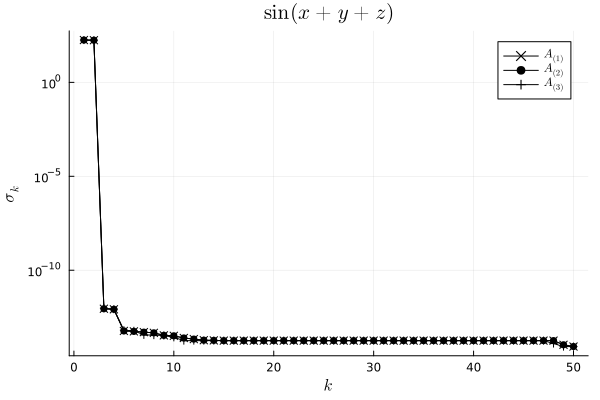
\includegraphics[width=\textwidth]{figures/lab3_e4_1.png}
    \caption{\label{fig:e41}}
  \end{subfigure}
  \hfill
  \begin{subfigure}{0.32\textwidth}
    \centering
    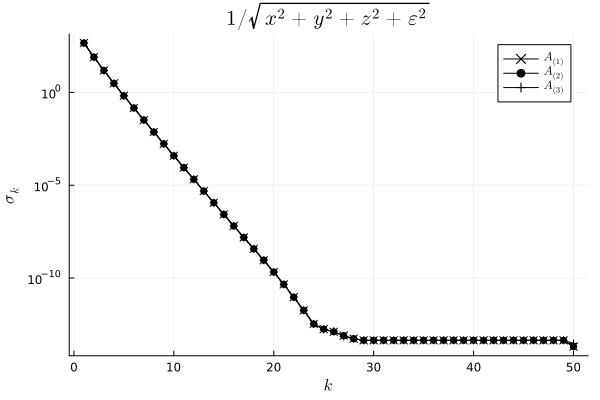
\includegraphics[width=\textwidth]{figures/lab3_e4_2.png}
    \caption{\label{fig:e42}}
  \end{subfigure}
  \begin{subfigure}{0.32\textwidth}
    \centering
    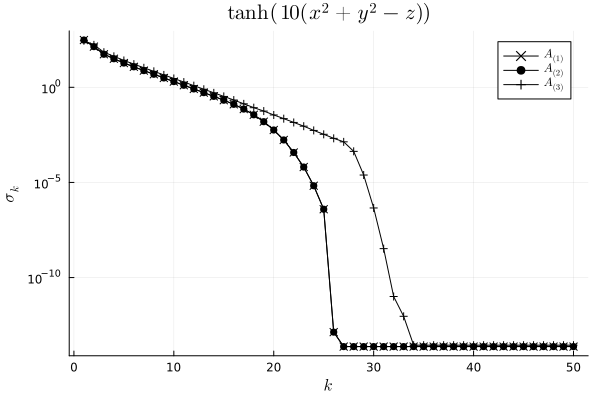
\includegraphics[width=\textwidth]{figures/lab3_e4_3.png}
    \caption{\label{fig:e43}}
  \end{subfigure}
  \caption{Plots for Exercise 4.\label{fig:e4}}
\end{figure}

\paragraph{Exercise 6}
Given are two Tucker tensors \[\mathcal{A}=[[\mathcal{G}; U_1, U_2,
  U_3]], \mathcal{B}=[[\mathcal{H}; V_1, V_2, V_3]] \quad \in
\mathbb{R}^{m\times n\times p},\] with core dimensions
\[\mathcal{G}\in \mathbb{R}^{q_1\times r_1 \times s_1},
\mathcal{H}\in \mathbb{R}^{q_2\times r_2 \times s_2}.\]
Consider the Tucker tensor \[\mathcal{C}=[[\mathcal{J}; W_1, W_2,
W_3]] \in \mathbb{R}^{m\times n\times p},\] with core dimension
\[\mathcal{J}\in \mathbb{R}^{(q_1+q_2)\times (r_1+r_2) \times (s_1+s_2)},\]
and the structure given by the following mode-1 unfolding:
\[J_{(1)}=
  \begin{bmatrix}G_{(1)} & 0_{q_2, r_1 s_1} & 0_{q_1, r_2
    s_1} & 0_{q_2, r_2 s_1} & 0_{q_1, r_1 s_2} &
    0_{q_2, r_1 s_2} & 0_{q_1, r_2 s_2} & H_{(1)}
\end{bmatrix}.\]
That is, in 3D, \(\mathcal{G}\) is located in the top left corner in
the front of \(\mathcal{J}\), while \(\mathcal{H}\) sits in the bottom
right corner in the back.
The factor matrices are given by
\[W_1 = [U_1 \, V_1],\; W_2 = [U_2 \, V_2], \; W_3 = [U_3 \, V_3].\]

For the implementation, it was crucial that I implement rounding as
described in~\cite{smith.etal_2026}.
As an example, consider adding a rank-1 tensor onto itself,
\(\mathcal{C}=\mathcal{A}+\mathcal{A}\).
After \verb|tucker_add()|, the factor matrices \(W_i = [U_i \, U_i]\)
will clearly be linearly dependent.
The procedure in the article applies, for each mode \(i\), a QR
decomposition to the factor matrices \(W_i = Q_i R_i\), then sets
\(\tilde{W}_i= Q_i\) and \(\tilde{\mathcal{G}} = \mathcal{G}\times_i R_i\).
This constitutes Phase 1 in their Algorithm 2.
As they write, this ``concentrates the
energy''~\cite[7]{smith.etal_2026} in the core.
Afterwards, I apply the procedure outlined in the lab
description to truncate the rank of \(\mathcal{C}\) (Phase 2).
\verb|l3ex6()| checks that this successfully recovers a rank-1 tensor
from adding two (and three) rank-1 tensors.

\begin{table}[h]
  \centering
  \begin{tabular}{l|l|l|l|l}
    \(\Delta t\)        & Time (A) & Time (B) & Error (A) & Error (B) \\
    \hline
    \(\Delta t^*\approx0.01\) & 0.14     & 0.62   & 0.22     & 0.22     \\
    \(\Delta t^* / 2\)  & 0.39     & 1.1    & 0.11     & 0.11     \\
    \(\Delta t^* / 4\)  & 0.45     & 2.5    & \num{3.5e-4}   & \num{1.4e-3}   \\
    \(\Delta t^* / 8\)  & 0.89     & 4.9    & \num{2.5e-2}   & \num{2.5e-2}
  \end{tabular}
  \caption{Error and time comparison of strategies A and
  B.\label{tab:strategies}}
\end{table}

\printbibliography{}

\end{document}
